\documentclass[12pt,a4paper]{article}
\usepackage[utf8]{inputenc}
\usepackage[brazil]{babel}
\usepackage[table]{xcolor}
\usepackage{graphicx}
\usepackage{color}
\usepackage{hyperref}
\usepackage{abnt-alf}
\usepackage[top=3cm,bottom=2cm,left=3cm,right=2cm]{geometry}
\usepackage{indentfirst}
\usepackage{float}

\begin{document}

% CAPA
\pagestyle{empty}
\begin{center}
\large  \textbf{UNIVERSIDADE PRESBITERIANA MACKENZIE}
\large  \textbf{PROGRAMA DE PÓS-GRADUAÇÃO EM}\\
\large  \textbf{ENGENHARIA ELÉTRICA E COMPUTAÇÃO}\\
\vskip 2.0cm
\textbf{\large Fernando Cainelli Tolentino}\\
\vskip 4.0cm
\setlength{\baselineskip}{1.5\baselineskip}
\textbf{\large Latent Dirichlet Allocation: Visualizando e Explorando Documentos   modelo generativo probabilístico}\\
\vskip 4.5cm
\end{center}
\hfill{\vbox{\hsize=8.5cm\noindent\strut
Projeto de Pesquisa apresentado ao Programa\break
de Pós-Graduação em Engenharia Elétrica e\break
Computação da Universidade Presbiteriana\break
Mackenzie como parte dos requisitos para a\break
aprovação na disciplina de Metodologia do\break
Trabalho Científico.}\\
\strut}
\vskip 3.0cm
\textbf{\normalsize Orientador: Prof. Dr. Leandro Augusto da Silva}\\
\vskip 2.0cm
\begin{center}
São Paulo\\
2017\\
\end{center}

% RESUMO
\newpage
\thispagestyle{plain}
\pagenumbering{roman}
\begin{center}
\large
\textbf{RESUMO}
\end{center}
\renewcommand{\baselinestretch}{0.6666666}

Considerando a quantidade de dados que se gera na atualidade e, que desse volume, grande parte está em formato de texto como e-mail, mensagens intântaneas, mídias sociais, websites e etc, há um crescente interesse  em nível tecnológico na interpretação desse tipo informação  que está disponível em um formato não estruturado. A interpretação consiste na elaboração estratégica para a descoberta de informação relevante nesse tipo de dado para uso em tomada de decisões. Uma abordagem para esta descoberta é com o uso do Latent Dirichlet Allocation (LDA), o qual consiste de um modelo generativo probabilístico que sumariza uma coleção de documentos em tópicos além de apresentar a relevância de cada tópico a cada
 documento. A interpretação e exploração de uma coleção de documentos pelo LDA pode ser feita a nível de tópico, palavra ou documento. LDAvis, por outro lado, consiste de um sistema para
 exploração de tópicos e palavras resultantes do modelo LDA. Este trabalho tem como objetivo estender as  funcionalidades do LDA para exploração do modelo a nível de documento e criação de relações de redes em mensagens de e-mail,
 promovendo uma ferramenta de busca aprimorada em um corpus.


% \begin{flushleft}
% {\bf Palavras-chave:} {\it apresentação, separada por vírgulas, de três a seis unitermos significativos para o trabalho.}
% \end{flushleft}

% SUMÁRIO
\newpage
\thispagestyle{empty}
\tableofcontents

% DESENVOLVIMENTO
\newpage
\pagestyle{plain}
\pagenumbering{arabic}
\renewcommand{\baselinestretch}{1.5}
\normalsize
\section{INTRODUÇÃO}
 
 Com acúmulo cada vez mais crescente de informações digitalizadas e armazenadas na forma de artigos, blogs, jornais, e-mails, livros, mensagens instantâneas, redes sociais, entre outros, 
 a tarefa de organizar, indexar e buscar esses tipos de informações torna-se uma tarefa fundamental para os usuários que precisam manipulá-las em um processo de tomada de decisão. 
 
 Para se ter como exemplo, pesquisas apontam que em 2017 uma média de 269 bilhões de e-mails serão enviados e recebidos diariamente, e espera-se continuar a crescer a uma taxa média de 4.4\% ao ano nos próximos quatro anos, atingindo 319.6 bilhões ao final de 2021 como mostra a Tabela \ref{tb_email} \cite{radicati2017}.

\begin{table}[h]
\label{tb_email}
  \centering
  \begin{tabular}{l*{6}{c}r}
  &					2017 &	2018 &	2019 &	2020 &	2021 & \\
  \hline
  Quantidade de E-mails &			269.0 &	281.1 &	293.6 &	306.4 &	319.6 & \\
  Crescimento(\%) &  	&		4.5\% &	4.4\% &	4.4\% &	4.3\% & \\
  \hline
  \end{tabular}
  \caption{Tráfego de Email Mundial Diário  (Bi). \cite{radicati2017}}
\end{table}

A taxa de crescimento da quantidade de mensagens enviadas e recebidas impressiona, não só por se tratar de uma técnologia dos anos 70,
mas principalmente pela forte adoção de novos recursos de comunicação como: mensagem instantânea, redes sociais, videoconferência, chat, etc. A comunicação via e-mail permanece sólida principalmente em empresas,
estas, por sua vez, tem a necessidade de aplicar a Inteligência nos Negócios (ou BI, de \textit{Business Intelligence}) para manter-se competitivas. O BI deve ser utilizado não só em escopos diretamente relacionados ao negócio,
como clientes, produtos, etc. mas também nos indiretos, como colaboradores, buscando obter insights, melhoria dos processos e otimização.
Frequentemente, e-mails são deixados fora da equação pela falta de ferramentas específicas e complexidade em tratar dados não estruturados,
 
 
 Retomando a discussão para a possibilidade de usuários navegar por grande volume de dados e encontrar a informação desejada, utiliza-se atualmente dois métodos principais:
 links e busca. 
 
 Os Links correlatam trechos de um documento a outro, sendo úteis pela possibilidade de permitir uma extensão da leitura e aprofundamento do conhecimento,
 direcionando o leitor a termos ou assuntos relacionados de alguma forma ao documento original. Apesar de ser uma maneira eficiente de fornecer conteúdo diretamente relacionado,
 existem desafios na aplicação do mesmo em escala, pois muitas vezes esse método é implementado de forma manual pelo autor. 
 
 A busca, por outro lado,
 requer um processo que pode ser automatizado de forma efetiva, pois quando informações presentes nos documentos são indexadas, possibilita ao usuário procurar um documento por palavra chave ou metadados presentes no mesmo.
 Esse processo é muito disseminado na área de recuperção de informação, e os motores de busca utilizam de técnicas combinadas como ranqueamento de resultados, aprendizagem de máquina e similaridade de palavras para melhorar a efetividade na busca de informações relevantes.

 O trabalho de \citeonline{mikolov2013efficient}, por exemplo, possibilita em um grande volume de documentos, fornecer funcionalidades como sugestões de termos de pesquisa baseados na ordem das palavras digitadas, além de extensão de busca utilizando termos similares.

Ambos os métodos têm a capacidade de uso na interação com os documentos, no entanto há uma lacuna quado se deseja explorar documentos por meio de temas de interesse específico,
 visualizar as palavras mais relevantes em cada tema e explorar os documentos com a usabilidade de um mapa, com possibilidade de ampliar a visualização com uso de zoom, além de visualizar a relação entre documentos de uma maneira intuitiva como pela proximidade. Estes exemplos de uso podem ser uma forma complementar ao métodos de links ou busca. E ainda, estes exemplos de aplicação podem ser feitos em qualquer corpus.
 
 %, no entanto, como exemplo,
 %vamos demonstrar como aplicação em um corpus contendo documentos de e-mail. E-mails possuem informações que podem aprimorar ainda mais a experiência de exploração,
 %pois os documentos podem ser exibidos em forma de nós, conectando remetentes a destinatários e aprimorando ainda mais a exibição dos resultados da pesquisa.

\subsection{OBJETIVOS}

Neste trabalho propõe-se como objetivo o uso de um algoritmo chamado Latent Dirichlet Allocation (LDA) para uso em problemas de visualização de modelos de tópicos \cite{blei2003latent}. A proposta consite em um aprimoramento da aplicação LDAVis de \citeonline{sievert2014ldavis} para explorar documentos e suas relações. O estudo de caso será feito em uma base de dados de e-mails e, após descoberta de tópicos, realizar a busca aprimorada de documentos, além de identificar  comunidades de redes de sociais através de interesse comum segundo os tópicos criados pelo modelo LDA. Além das técnicas de processamento e visualização de conhecimento, como objetivo secundário propõe-se realizar análise exploratória do conjunto de dados para obter informações relevantes e que possam ser utilizadas na compreensão do negócio da empresa.


\subsection{ORGANIZAÇÃO DO TRABALHO}

 A estrutura organizacional dessa dissertação consiste em 5 capítulos. O capítulo 1, segue com uma breve introdução e organização do trabalho. 
  No capítulo 2, justificamos a elaboração do trabalho demonstrando que a visualização de modelos de tópicos é uma das áreas em carência de pesquisa atualmente, 
  e como esse trabalho busca contribuir com o campo de \textit{Information Retrival} para modelos de tópicos. No capítulo 3, discorremos sobre o referencial teórico presente, 
  é detalhado o funcionamento do modelo probabilístico LDA além da apresentação do algoritmo K-Means como base de comparação. No capítulo 4, mostramos a metodologia adotada, 
  a arquitetura, o processo de mineração de dados, as justificativas de adoção de cada parâmetro livre na criação do modelo além das funcionalidades propostas para
  aplicação de busca. Por fim, no capítulo 5, apresentamos o cronograma com as tarefas pendentes para a conclusão do trabalho.


% JUSTIFICATIVA


% REFERENCIAL TEÓRICO
%\section{REFERENCIAL TEÓRICO}
%No campo de processamento de linguagem natural e recuperação de informação, existem diversas técnicas de agrupamento, análise e extração de sentido de um conjunto de dados de textos.Nesta seção, vamos apresentar as técnicas disponíveis e trabalhos relatos relevantes utilizados neste artigo.



% K-MEANS
%\subsection{K-MEANS}
%O algoritmo K-Means, assinala a cada objeto de um conjunto de dados a um grupo, foi introduzido inicialmente por \citeonline{macqueen1967some} e é um dos algoritmos mais estudados na literatura.
 
 %O algoritmo é inicializado com dois parâmetros principais, o número de clusters, ou grupos, disponíveis para os objetos no dataset serem classificados e um vetor de objetos que representa o conjunto de dados.
 
 %Cada objeto no conjunto de dados pode ser assinalado a um grupo a cada iteração. Primeiro determinamos os centróides iniciais, centróides são a representação de um grupo e seu valor é dado pela média dos objetos desse grupo, são iniciados randomicamente, como proposto  pelo trabalho original,ou utilizando algum algoritmo de otimização, em alguns casos, o K-Means pode convergir para grupos distintos dependendo do valor inicial dos centróides. 
 
 %Existem diversos estudos que adotam diferentes algoritmos e técnicas para inicialização dos centróides,\citeonline{yuan2004new} propuseram um método para se obter os centróides iniciais de acordo com a distribuição do conjunto de dados,em sua pesquisa obtiveram melhor acurácia com essa técnica quando comparada a inicialização randômica proposta no trabalho original de \citeonline{macqueen1967some}.

%O próximo passo é rodar o algoritmo até que convirja. Para cada iteração,o algoritmo assinala cada objeto ao grupo cujo centróide está mais próximo e calcula a nova média do grupo para então ajustar os valores dos centróides.Para determinar a distância entre um objeto observado e os centróides, K-Means utiliza a distância Euclidiana que calcula a diferença entre um objeto vetor \(X=(x_1, x_2... x_n)\) e um centróide vetor \(C=(c_1, c_2... c_n)\) com a seguinte fórmula: 

%\begin{equation}
%d(X,C) = \sqrt{(x_1 - c_1)^2 + (x_2 - c_2)^2 ... + (x_n - %c_n)^2}
%\end{equation}

%O objeto $X$ será assinalado ao grupo cujo centróide tem a menor distância Euclidiana. Em seguida, o algoritmo percorre cada grupo calculando a média dos objetos nele presente,e define esse valor ao centróide do grupo. O processo se repete até que os objetos não troquem de grupo.

%O algoritmo K-Means assinala cada objeto do conjunto de dados a exatamente um grupo, no entanto, para problemas que objetos podem pertencer a mais de um grupo,ou quando grupos de dados são representados por uma forma não circular, uma vez que é  utilizada a distância Euclidiana para assinalar objetos a grupos, um modelo misto, ou mixture model,podem obter agrupamentos com melhores representações.



%% LATENT DIRICHLET ALLOCATION
%\subsection{LATENT DIRICHLET ALLOCATION}
\section{LATENT DIRICHLET ALLOCATION}
Latent Dirichlet Allocation, ou LDA, é um modelo generativo probabilístico proposto por \citeonline{blei2003latent} e usado em diversas áreas como análise de sentimento,
 classificação de documentos, bioinformática, agrupamento de dados entre outros. 
 
 O resultado do LDA sugere que palavras de uma coleção de documentos carregam uma forte informação semântica,
 e que documentos com assuntos similares contém também um grupo de palavras similares. Os tópicos latentes, ou ocultos,
 são portanto descobertos pelo algoritmo, identificando o grupo de palavras no corpus que co-ocorrem frequentemente dentro dos documentos. As premissas  básicas do LDA são:

\begin{enumerate}
  \item cada documento é representado por uma mescla de tópicos;
  \item cada tópico é formado por uma distribuição de palavras.
\end{enumerate}

O objetivo do algoritmo LDA é encontrar o modelo probabilístico de um conjunto de dados. Essa característica o difere das abosrdagens de Mistura de Unigramas, os quais assumem que cada documento exibe características de apenas um tópico. Ou seja, o modelo resultante do LDA  permite que documentos contenham múltiplos tópicos ao mesmo tempo e com relevância distintas. Nesta seção, discorre-se sobre as principais características do trabalho original de \citeonline{blei2003latent}.
 
 A pesquisa de \citeonline{hu2009latent} foi complementar durante essa seção para melhor compreender o trabalho original.

%Antes de nos aprofundarmos na descrição do algoritmo, façamos uma introdução da terminologia formal e notações usada nesta seção.


%% PROCESSO GENERATIVO
\subsection{PROCESSO GENERATIVO}

Em uma análise textual, que é mais ampla a análise de  tópicos, uma $palavra$ é a unidade mais básica de dado, definida com um item de um vocabulário indexado por \(w \in \{1,. . . , V\}\)  , onde $V$ é o número de palavras únicas dentro de um corpus, também denominado vocabulário. As palavras são representadas como um vetor de base unitária.Assim, um documento é uma sequência de $N$ palavras denotadas por \(\textbf{ w} = (w_1, w_2,. . . ,  w_N)\). Por fim, um corpus é uma coleção de $M$ documentos denotados por \(\textbf{ D} = \{\textbf{ w}_1, \textbf{ w}_2, . . ., \textbf{ w}_M\}\).

\underline{O LDA assume que documentos são criados via um processo generativo no qual palavras nos documentos são geradas. Com base no tamanho do documento,
 nós escolhamos uma mistura de tópicos usando a distribuição multinomial de tópicos para escolher as palavras que devem ser usadas para preencher a cota de cada tópico}. Por exemplo, dado um conjunto de documentos que podem ser classificados em quatro tópicos: Esportes, Animais, Tecnologia e Artes. Cada tópico poderá ser definido pela seguinte lista de palavras:

\begin{itemize}
  \item \textbf{ Esportes:} bola, futebol, basquete, gol, pontos, corrida, natação.
  \item \textbf{ Animais:} coelho, cachorro, gato, galinha, touro, aranha.
  \item \textbf{ Tecnologia:} computadores, smartphone, tablet, tech, câmera, web.
  \item \textbf{ Artes:} cinema, dança, música, canção, pintura, cores, movimento, instrumento.
\end{itemize}

O processo generativo consiste em uma mistura de tópicos com base em uma parametrização feita pelo usuário. No caso do exemplo acima, suponha-se que há um desejo em gerar um novo documento que contenha os seguintes tópicos nas respctivas proporções: 75\% Artes e 25\% Esporte. A geração inicia-se com a parametrização do tamanho do documento a ser gerado pelo número de palavras. Consequentemente, para cada tópico escolhido na mistura, seleciona-se as palavras de cada tópico proporcionalmente, gerando o novo documento.

 O LDA usa esse conceito de processo generativo de forma reversa para determinar a distribuição de tópicos por documento e a distribuição de palavras por um tópico. 
 O processo generativo permite diferentes graus de relevância de uma palavra em um tópico, e um tópico em um documento. Na teoria da probabilidade isso é chamado como permutabilidade,
 ou exchangeability \cite{aldous1985exchangeability}. 
 
 Para cada documento indexado por $d \in \{1,. . . , M\}$ em um corpus $D$, o processo generativo pode ser formalmente descrito da seguinte maneira:


\begin{enumerate}
  \item Escolha um vetor de tópico $\theta _d$ de dimensão $K$ da distribuição $p(\theta|\alpha)=Dirichlet(\alpha)$.
  \item Para cada uma das $N$ palavras ($w_n$) dentro de um documento:
  \begin{enumerate}
  	\item Escolha um tópico \(z_n \in \{1,. . . , K\}\) do Multinômio ($\theta$).
    \item Escolha uma palavra $w_n$ de \(p(w_n=1| z_n=j,\beta)=\beta _{ij}\), que é a distribuição probabilística multinomial condicionada ao tópico $z_n$.
  \end{enumerate}
\end{enumerate}

% O  hiper parâmetro $\alpha$ é um vetor de dimensão $K$ com itens \(\alpha _i>0\) e é uma distribuição Dirichlet priori da distribuição de tópicos por documento,
%  o hiper parâmetro $\beta$ é uma distribuição Dirichlet priori da distribuição de palavras por tópicos. $\theta _d$ é a distribuição de tópicos para o documento $d$. $Z_{dn}$ e $W_{dn}$ são as variáveis a nível de palavras e são amostradas uma vez para cada palavra em cada documento.

Uma variável de distribuição Dirichlet randômica $\theta$ com dimensão $K$ tem como propriedade: $\theta ^i \geq 0, \displaystyle\sum_{i=1}^{K} \theta ^i = 1$ e têm a seguinte densidade probabilística:

\begin{equation}
p(\theta|\alpha) = \frac{\Gamma(\displaystyle\sum_{i=1}^{K} \alpha _i)}{\displaystyle\prod_{i=1}^{K} \Gamma(\alpha _i)} \theta _1 ^{\alpha _i - 1} ...  \theta _K ^{\alpha _K - 1}
\end{equation}

A distribuição Dirichlet é utilizada por essa possuir um conjunto de propriedades importantes que possibilita um processo de inferência e estimação de parâmetros mais simples.
 A distribuição é da família exponencial, conjuga com a distribuição multinomial, possui dimensões finitas e possui estatística suficiente.
 A distribuição  acima dá a cada documento seu próprio vetor de distribuição que indica a relevância de cada tópico $K$ a aquele documento.
 Assim, o processo generativo descrito acima define a distribuição conjunta para cada documento $\textbf{ w}_d$.

Dado os hiper parâmetros $\alpha$ e $\beta$, a distribuição conjunta de uma mistura de tópico $\theta$ e um conjunto de $N$ tópicos $z$ é dado por:

\begin{equation}
p(\theta,\textbf{z},\textbf{w}|\alpha,\beta) = p(\theta|\alpha) \prod_{n=1}^{N} p(z_n|\theta)p(w_n|z_n,\beta)
\end{equation}

onde $p(z_n | \theta)$ é simplesmente $\theta _i$ para cada $i$ único,
 tal que, $z_{ni}=1$.
 
A obtenção da distribuição marginal de um documento $\textbf{w}$ é dada a partir da integração sobre $\theta$ e somando sobre $z$:

\begin{equation}
p(\textbf{w}|\alpha,\beta)=\int{p(\theta|\alpha)\Bigg(\prod_{n=1}^{N}\sum_{z_n} p(z_n|\theta)p(w_n|z_n,\beta)\Bigg)d\theta},
\end{equation}

e finalmente, a distribuição de probabilidade do corpus $D$ é obtida com o produto das probabilidades marginais de um documento:

\begin{equation}
p(D|\alpha,\beta)= \prod_{d=1}^{M} \int{p(\theta _d|\alpha)\Bigg(\prod_{n=1}^{N_d}\sum_{z_{dn}} p(z_{dn}|\theta _d)p(w_{dn}|z_{dn},\beta)\Bigg)d\theta _d}
\end{equation}


A Figura \ref{fig-plate} ilustra o 	\textit{Plate Notation} do modelo LDA, as caixas são pratos representando réplicas,
o $M$ denota o número de documentos que é associado ao prato externo e o interno representa as palavras dentro de um documento, onde $N$ denota o número de palavras.

\begin{figure}[H]
 \centering
   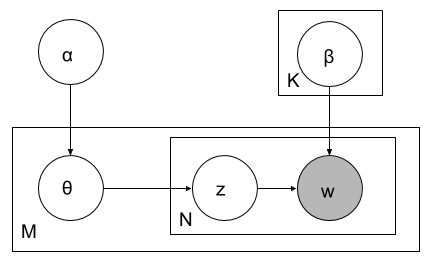
\includegraphics[height=10cm]{images/figure_1.png}
   \caption{Plate Notation representando o modelo LDA, adaptado de \citeonline{blei2003latent}}
   \label{fig-plate}
\end{figure}

O hiper parâmetro $\alpha$ é um vetor de dimensão $K$ com itens \(\alpha _i>0\) e é uma distribuição Dirichlet apriori da distribuição de tópicos por documento,
o hiper parâmetro $\beta$ é uma distribuição Dirichlet apriori da distribuição de palavras por tópicos. $\theta _d$ é a distribuição de tópicos para o documento $d$. $Z_{dn}$ e $W_{dn}$ são as variáveis a nível de palavras e são amostradas uma vez para cada palavra em cada documento.


%% INFERÊNCIA
\subsection{INFERÊNCIA}
A Eq.(3) baseia-se nos hiper parâmetros apriori $\alpha$ e $\beta$, nesta seção, descreve-se o procedimento para inferência com o LDA.

O problema de inferência principal a se resolver é o de se computar a distribuição posteriori das distribuições latentes:

\begin{equation}
p(\theta,\textbf{z}|\textbf{w},\alpha,\beta) = \frac{p(\theta,\textbf{z},\textbf{w}|\alpha,\beta)}{p(\textbf{w}|\alpha,\beta)}
\end{equation}

A distribuição acima é intratável de se computar em geral, o numerador é a distribuição conjunta das variáveis randômicas, que são computáveis para qualquer configuração de variáveis ocultas,
 o denominador é a distribuição marginal, em teoria, pode ser calculada somando a distribuição conjunta de todas instâncias possíveis. No entanto,
 o número de estruturas de tópicos é exponencial e essa soma é intratável de se computar \cite{blei2012probabilistic}. Para normalizar a distribuição da Eq.(4) é utilizado a distribuição marginal,
 de todos os documentos em um corpus:

\begin{equation}
p(\textbf{w}|\alpha,\beta)=\frac{\Gamma(\sum_{i}\alpha_i)}{\prod_{i}\Gamma(\alpha_i)}\int{\Bigg(\prod_{i=1}^{K}\theta_i^{\alpha_i-1}\Bigg)} \Bigg(\prod_{n=1}^{N}\sum_{i=1}^{K}\prod_{j=1}^{V}(\theta_i\beta_{ij})^{w_n^j}\Bigg)d\theta
\end{equation}

Embora a distribuição posterior é intratável devido ao acoplamento do $\theta$ e $\beta$, existe uma variedade de algoritmos de aproximação de inferência que podem ser usados. Os métodos comumente encontrados na literatura são baseados em amostragem ou variação.

O algoritmo de amostragem mais comum para modelação de tópicos é o Gibbs Sampling, uma instanciação especial da Cadeia de Markov Monte Carlo (MCMC) \cite{jordan1999introduction},
 uma sequência de variáveis randômicas, uma dependente da anterior. O algoritmo roda coletando amostras da distribuição assintótica e então aproximando a distribuição com as amostras coletadas.
 O problema reside em não saber ao certo  quando o algoritmo convergiu para solução, além dos seus requisitos de memória, já que escala linearmente com o número de palavras em um corpus,
 isso torna o algoritmo não adotável em uma conjunto de dados muito grande \cite{vrehuuvrek2011scalability}.

O método mais utilizado em modelos de variável latente é o algoritmo variacional Expectation-Maximization(EM), que permite a estimação de parâmetros não supervisionada de maneira computacionalmente eficiente. O método determinístico de aproximação EM resulta em uma estimativa tendenciosa. Em cada iteração é atualizado os parâmetros computando os valores esperados das variáveis sobre a distribuição posterior na Eq.(7).


\begin{figure}[H]
	\centering
    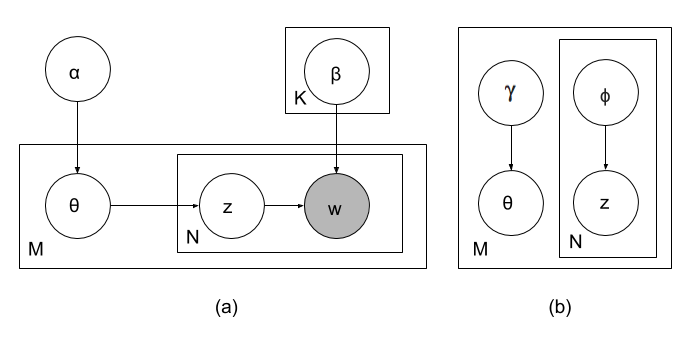
\includegraphics[height=10cm]{images/figure_2.png}
    \caption{(a) Representação gráfica do modelo LDA. (b) A aproximação variacional para a distribuição posteriori. Adaptado de \citeonline{blei2003latent}}
\end{figure}

A ideia do trabalho original de utilizar inferência variacional baseada na convexidade é de se fazer o uso da desigualdade de Jensen para obter um limite inferior ajustável na verossimilhança \cite{jordan1999introduction} onde os parâmetros variacionais são escolhidos através de um processo de otimização,
 tentando encontrar o limite inferior mais próximo em cada iteração. Considerando a Figura 2(a), a problemática do acoplamento dos parâmetros $\theta$ e $\beta$ surge devido às bordas entre $\theta$, $z$,
 e nó $w$, removendo-os, assim como se faz com as dependências entre as variáveis que tornam a equação intratável. Com isso,
 resulta-se em um Plate Notation simplificado com parâmetros variacionais livres como ilustrados na Figura 2(b), obtendo a família de distribuição de probabilidade nas variáveis ocultas,
 que é caracterizada pela seguinte distribuição variacional:

\begin{equation}
q(\theta,\textbf{z}|\gamma,\phi)=q(\theta|\gamma)\prod_{n=1}^{N}q(z_n|\phi_n), 
\end{equation}

onde a distribuição  $q(\gamma|\phi)$ é a distribuição Dirichlet com parâmetro variacional $\gamma_d$, mostrando a distribuição dos tópicos em cada documento.
 As distribuições $q(z_n | \phi_n)$ são multinomiais com parâmetros variacionais $\phi_n$ e existem a nível de palavras, onde $\phi_{ni}$ é a probabilidade que a $n_{gesima}$ palavra foi gerada pelo $i_{gesimo}$ tópico oculto.

O próximo passo é configurar um problema de otimização que determina os parâmetros $\gamma$ e $\phi$. Os valores ideais são encontrados minimizando a divergência Kullback Leibler(KL) entre a distribuição posterior $p(\theta, z|w,\alpha,\beta)$ e a distribuição variacional.
 O par de equações de atualização resultantes segundo \citeonline{blei2003latent} são:

\begin{equation}
\phi_{ni} \propto \beta_{iwn} exp\{E_q[log(\theta_i)|\gamma]\}
\end{equation}

\begin{equation}
\gamma_i = \alpha_i + \sum_{n=1}^{N} \phi_{ni}
\end{equation}

As equações acima são utilizadas no algoritmo EM para estimativa dos parâmetros. Esse processo é descrito na sequência.

%% ESTIMAçÃO DE PARÂMETROS
\subsection{ESTIMAÇÃO DE PARÂMETROS}
Dado um corpus contendo documentos $\textbf{D} = \{\textbf{w}_1, \textbf{w}_2, . . ., \textbf{w}_M\}$ os valores ideais dos hiper parâmetros $\alpha$ e $\beta$
 que maximizam a verossimilhança de todos documentos $\textbf{w}$ em um corpus $D$ é dado por:

\begin{equation}
l(\alpha|\beta) = \sum_{d=1}^{M} log\ p(\textbf{w}_d|\alpha,\beta)
\end{equation}

O valor de $l(\alpha, \beta)$ pode ser computado se o valor de $p(\textbf{w}_d|\alpha, \beta)$ é conhecido para cada documento $d$. No entanto,
 como descrito acima, $p(\textbf{w}|\alpha,\beta)$ não pode ser computado. Então utiliza-se o limite inferior na função de verossimilhança.
 O EM então estima os hiper parâmetros $\alpha$ e $\beta$ para maximizar esse limite enquanto corrige os parâmetros variacionais $\gamma$ e $\phi$. 
 O algoritmo variacional EM continua iterativamente em dois passos:

\begin{enumerate}
\item \textbf{Passo-E:} Para cada documento $d \in \{1,. . . , M\}$, os parâmetros variacionais $\gamma_d$ e $\phi_d$ são estimados maximizando a verossimilhança utilizando o limite inferior descrito na seção anterior.
\item \textbf{Passo-M:} O limite inferior é maximizado  de acordo com os hiper parâmetros $\alpha$ e $\beta$ do modelo para se obter os novos valores. 
 Isso corresponde a encontrar a máxima verossimilhança com estatísticas suficientes esperadas para cada documento sob a aproximação posteriori.
\end{enumerate}

Os passos acima são repetidos até que o limite inferior da verossimilhança convirja. Como resultado final obtém-se duas matrizes $V \times K$ e $M \times K$,
 representando  a distribuição de palavras em cada tópico e a distribuição de tópicos em cada documento, respectivamente.



%% METODOLOGIA
\section{METODOLOGIA}
O conjunto de dados utilizado a ser utilizado neste trabalho trata-se de uma coleção de e-mails retirados de um ambiente real de uma empresa provedora de serviços. 
 Para os experimentos realizados neste trabalho foram coletados 100.000 mensagens de e-mail. No geral, essas mensagens de e-mail seguem as RFCs 822, 2045, 2046, 2047, 4288, 4289 e 2049,
 que são os padrões da indústria para troca de e-mails.	Em resumo, as mensagens são formadas por headers contendo informações sobre assunto, remetente, destinatários e data.
 Existem também headers contento outros tipos de informações como caminho percorrido pela mensagem até o seu destino final, análises de filtro de conteúdo entre outros. Esses geralmente relevantes a administradores do serviço. O corpo e-mail contém o conteúdo da mensagem em si, que pode ser segmentado em  partes, cada uma com seu próprio content-type. 
 Os content-types mais comuns entre mensagens de e-mail são: text/plain, text/html, multipart/mixed, application/octet-stream entre outros, esses se referem ao tipo do conteúdo seguinte no corpo do e-mail.
 Essa informação é utilizada por clientes de e-mail para decodificar adequadamente a mensagem. Dessa forma é possível realizar o download de arquivos separadamente ou renderizar imagens ou conteúdo html dentro da mensagem.


%% PARSER
\subsection{PARSER}
Para cada mensagem processada é aplicado um conjunto de filtros, normatizações e presunções com o intuito de se obter a mais fiel e relevante representação vetorial do documento.
 Para isso, foram adotados processos adotados em mineração de textos, descritos abaixo:

\begin{enumerate}
\item \textbf{Pré-processamento:} Nesse passo, utilizou-se a biblioteca Flanker, \citeonline{flanker2017}, para primeira estruturação do documento, fazendo o parsing dos headers de interesse. Nesse passo são extraídos os valores dos headers ‘Subject’, ‘Date’, ‘From’, ‘To’, ‘Cc’, ‘X-Spam-Flag’ essas informações não são utilizadas para a geração do modelo,
 no entanto são informações complementares e serão úteis na análise exploratória e busca dos documentos. Se a mensagem for classificada como spam, ou seja, 
 se o valor do header X-Spam-Flag for igual a ‘YES’ ou o assunto da mensagem conter a palavra ‘spam’, \textit{case insensitive}, a mensagem será descartada e não será utilizada para criação do modelo,
 uma vez que temos interesse apenas em mensagens legítimas. O body do documento é dividido em múltiplas partes, cada parte possui seu próprio content-type,
 são processadas as partes com conteúdos de tipo text/html e text/plain, descartando anexos, mensagens criptografadas e codificadas. 
 Para conteúdos do tipo text/html são removidas todas as tags e propriedades html e css presentes via expressões regulares.
\item \textbf{Bag of Words:} Usando o texto extraído do body na etapa acima é criado uma bag of words a partir do documento, que é a representação vetorial desse texto,
 onde os elementos são as palavras presentes no texto, aqui é desconsiderado ordem ou gramática, no entanto, a multiplicidade é perene.
\item \textbf{Stop Words:} Stop words são uma lista de palavras comumente utilizadas em determinada língua, elas não são um indicador relevante na representação de um tópico.
 Esse passo remove as stop words presentes no dicionário Português e Inglês pois são as línguas presentes na coleção de documentos de e-mail.
\item \textbf{Stemming:} Todas as palavras são convertidas para letras minúsculas e é então aplicado o algoritmo de stemming de \citeonline{porter1980algorithm}
 na implementação da biblioteca NLTK(Natural Language Toolkit) \citeonline{Bird:2009:NLP:1717171} para remover afixos morfológicos das palavras, reduzindo-as ao seu radical, como exemplificado na Tabela \ref{tab-stem}.


\begin{table}[h]
  \centering
  \begin{tabular}{l l l}
  Palavra		&Stem &\\
  \hline
  copiar		&copi &\\
  copiando		&copi &\\
  copiou		&copi &\\
  \hline
  \end{tabular}
  \caption{Palavra original e seu respectivo Steam}
  \label{tab-stem}
\end{table}

Na Tabela \ref{tab-stem}, nota-se a redução no número de palavras únicas aplicando o steam. O número de palavras únicas em um conjunto de documentos afeta diretamente o tempo de execução na criação do modelo LDA.
 Por outro lado, a redução pode causar um efeito não desejado distorcendo o sentido das palavra. Na seção de resultados apresenta-se a diferença entre a aplicação ou não desse processo na coleção de documentos de e-mail utilizado.
\end{enumerate}


O processo acima resulta na mensagem original, seus metadados e a bag of words com os termos presentes no texto. Esses dados são armazenados e indexados no Elasticsearch,
 um dos motores de busca open-source mais adotados atualmente. Esse processo possibilita a busca por palavras, frases, destinatários, remetentes e data. 

Em trabalhos semelhantes como \citeonline{ozcaglar2008classification} é possível notar que muitas técnicas empregadas nessa fase são comuns, porém, uma das principais diferenças,
 é a aplicação de processos mais detalhados na estruturação e armazenamento dos metadados, pois esses são fundamentais na análise exploratória dos documentos.
 \citeonline{ozcaglar2008classification} não se aprofunda nesses aspectos, pois tais informações não eram relevantes ao escopo da sua pesquisa,
 porém, como trabalhos futuros, sugeriu justamente a exploração de comunidades baseada em interesses dos destinatários e remetentes, o que demonstraremos possível na aplicação proposta.

O próximo passo é a criação do modelo para representar esse conjunto de dados e aprimorar a representação de um documento.



%% CRIAÇÃO DO MODELO
\subsection{CRIAÇÃO DO MODELO}
O conjunto de dados é carregado do Elasticsearch, nessa fase, são requeridos os tokens dos documentos gerados no processo de parsing, então
 um filtro é aplicado na query de busca para retornar apenas esses resultados. A coleção de tokens é convertida em uma matriz de contadores de tokens onde o número de features será igual ao tamanho do vocabulário, como se pode verificar na Tabela \ref{tab-voc}.


\begin{table}[h]
  \centering
  \begin{tabular}{l l l}
  Tokens		&Vetor &\\
  \hline
  $Array(word_1, word_2, word_3, word_n)$						&(n,[0,1,2,n], [1.0, 1.0, 1.0, 1.0]) &\\
  $Array(word_1, word_2, word_2, word_3, word_1)$				&(n,[0,1,2,n], [2.0, 2.0, 1.0, 0.0]) &\\
  $Array(word_2, word_3, word_2, word_n)$						&(n,[0,1,2,n], [0.0, 2.0, 1.0, 1.0]) &\\
  \hline
  \end{tabular}
  
  \caption{Conversão de tokens de palavras para vetor de contadores}
  \label{tab-voc}
\end{table}


Na Tabela \ref{tab-voc} pode-se ver uma representação da saída esperada. É criado uma matriz de frequência de termos $M \times N$, para cada documento,
 $d \in \{1,. . . , M\}$ é criado uma representação vetorial do vocabulário do corpus($N$), que contém a frequência da palavra no documento em sua respectiva posição nesse vetor.
 Esse formato é requerido como formato de entrada dos dados para o modelo LDA.

O parâmetro $\alpha$ do algoritmo é a priori da distribuição de tópicos por documento ($\theta$) e o parâmetro $\eta$ é a priori da distribuição de palavras por tópico ($\beta$),
 através desses parâmetros, é possível tendenciar o modelo para que determinadas palavras sejam mais relevantes a alguns tópicos à outros,
 além de possibilitar que um grupo de documentos com a mesma característica sejam definidos com uma distribuição similar entre si e distintas dos demais,
 tendenciando-os a uma relevância maior a um ou mais tópicos. De forma a não tendenciar o modelo, optou-se por uma distribuição uniforme desses parâmetros,
 para isso normalizamos essas distribuições definindo $\alpha$ e $\beta$ como $\frac{1}{K}$.

Como último parâmetro, precisa-se definir o número $K$ de tópicos desejados. Existem algumas formas para encontrar o melhor parâmetro $K$.  \citeonline{ozcaglar2008classification}, por exemplo, utilizou o Erro Quadrático para definir seu número otimizado de tópicos. Pesquisas recentes, no entanto,
 propõe o uso da medida de coerência proposta por \citeonline{roder2015exploring} para mensurar a qualidade de um tópico. O processo é dado por quatro fases descritas na Figura \ref{fig-proc}, a saber:


\begin{figure}[H]
	\centering
    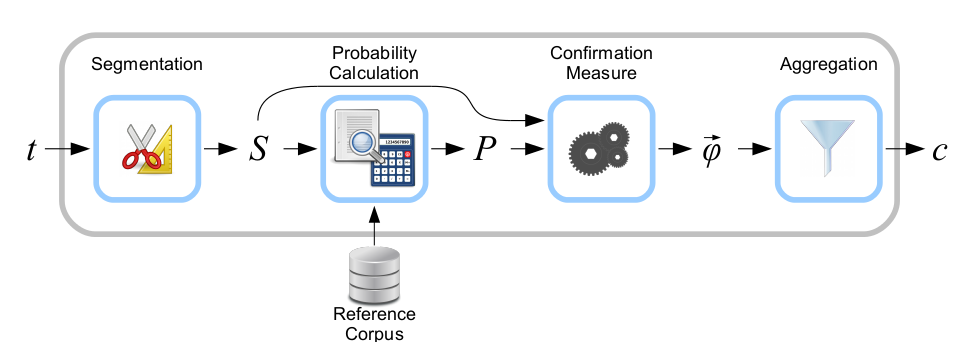
\includegraphics[height=5cm]{images/figure_3.png}
    \caption{Visão geral do framework de mensuração da coerência dos tópicos. Imagem original \citeonline{roder2015exploring}}
    \label{fig-proc}

\end{figure}


\begin{enumerate}
\item \textbf{Segmentação:} Para cada tópico $t \in \{1 ... K\}$ é extraído um conjunto de palavras mais relevantes de acordo com o modelo resultante,
 então é criado pares combinatórios distintos entre essas palavras. Veja exemplo na Figura \ref{fig-exe}.

\begin{table}[h]
  \centering
  \begin{tabular}{l l l l l l l l l}
  & & &0 &1 &2 &3 &4 &5 \\
  \hline
  &Tópico &3 &dados &máquina &mineração &neurais &redes &aprendizagem \\
  \hline
  \end{tabular}
  \caption{Representação de um tópico e suas palavras mais relevantes}
  \label{fig-exe}
\end{table}

No exemplo da Figura \ref{fig-exe} observa-se um único tópico e as palavras com maior probabilidade de pertencerem ao mesmo. É gerado a partir dessas palavras bigramas de palavras $S_i$, como:

\[\{(m\acute{a}quina, dados),\ (aprendizagem, m\acute{a}quina),\ (neurais, redes),\ ...\}\]

Formalmente os bigramas são formados da seguinte maneira:

\begin{equation}
S_{um}^{um} = \{(W',W^*)|W' = \{w_i\};
W^* =  \{w_j\};w_i,w_j \in W; i \neq j\}
\end{equation}

\begin{equation}
S_{anterior}^{um} = \{(W',W^*)|W' = \{w_i\};
W^* =  \{w_j\};w_i,w_j \in W; i > j\}
\end{equation}

\begin{equation}
S_{posterior}^{um} = \{(W',W^*)|W' = \{w_i\};
W^* =  \{w_j\};w_i,w_j \in W; i < j\}
\end{equation}

As duas últimas são variações da primeira que requer um conjunto ordenado, elas comparam uma palavra apenas com sua palavra anterior e posterior respectivamente, \cite{roder2015exploring}.

\item \textbf{Cálculo de Probabilidade:} É calculado a probabilidade das palavras ocorrerem de forma conjunta. O cálculo é feito da seguinte maneira:

\[P(w_i,w_j) = \frac{N\acute{u}mero\ de\ documentos\ que\ cont\acute{e}m\ palavras\ w_i\ e\ w_j}{Total\ de\ documentos}\]

\item \textbf{Medida de Confirmação:} A medida de confirmação recebe um único par $S_i = (W',W^*)$, ou subconjunto de palavras bem como suas respectivas probabilidades
 para calcular o quão forte o conjunto de palavras condicionais $W^*$ suporta $W'$

\item \textbf{Agregação:} Por fim, todas as confirmações de todos conjuntos de pares $S_i$ são agregados em uma única pontuação de coerência pela sua média.
\end{enumerate}

O LDA foi inicialmente experimentado em conjuntos de dados com 4, 8, 16, 32, 64 e 128 tópicos e parâmetros $\eta$ e $\alpha$ com distribuições uniformes. Para cada configuração de parâmetro $K$,
 obteve-se a pontuação de coerência do modelo via processo descrito acima. O valor de $K$ utilizado foi o que obteve maior coerência.

Por fim, selecionou-se as distribuições do modelo gerado com a configuração de $K$ otimizada, e então adicionou-se um novo metadado para cada documento armazenado no Elasticsearch com sua distribuição de tópicos.
 Também foi armazenado em uma outra estrutura a distribuição de palavras por tópico. Essas informações serão utilizadas no processo de visualização.

%% APLICAÇÃO
\subsection{APLICAÇÃO}
A aplicação web interativa é uma extensão do LDAvis \cite{sievert2014ldavis}, o trabalho original tem duas funcionalidades principais
que permitem ao usuário explorar o modelo.

\begin{figure}[H]
	\centering
    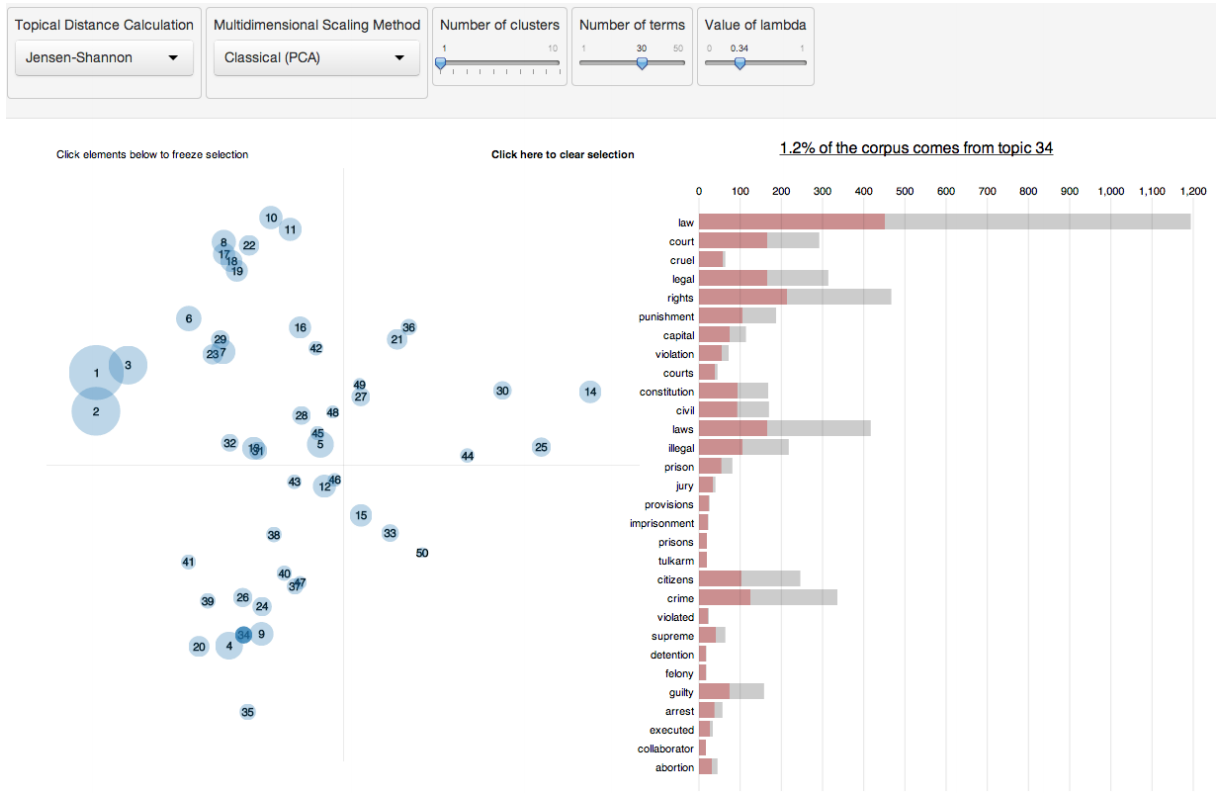
\includegraphics[height=10cm]{images/figure_4.png}
    \caption{Layout do LDAvis. A esquerda a visualização de tópicos e a direita o gráfico de barras com o tópico 34 selecionado. Imagem do trabalho original \cite{sievert2014ldavis}}
\end{figure}


\begin{enumerate}
  \item Possibilita o usuário selecionar um tópico e visualizar os termos mais relevantes dentro dele.
  \item Possibilita o usuário selecionar um termo para revelar sua distribuição condicional sobre os tópicos. Essa distribuição
  é visualizada alterando a área dos círculos tal que seja proporcional a frequência do termo selecionado.
\end{enumerate}

A proposta é estender a visualização para exploração não apenas dos tópicos e palavras mas também dos documentos. Ao final do desenvolvimento esperamos entregar as seguintes funcionalidades extras:

\begin{enumerate}
  \item Busca de documentos:
  \begin{enumerate}
    \item Por palavra.
    \item Por trechos de palavras.
    \item Por data.
    \item Por remetente.
    \item Por destinatários.
    \item Por tópico mais relevante.
  \end{enumerate}
  \item Visualização de comunidades:
  \begin{enumerate}
    \item Por interesse em tópicos comuns.
    \item Por interesse em documentos comuns.
  \end{enumerate}
  \item Análise exploratória do conjunto de dados.
  \begin{enumerate}
    \item Quantidade de documentos por tópico.
    \item Quantidade de usuários.
    \item Usuários mais relevantes por tópico
  \end{enumerate}
\end{enumerate}

Os documentos são indexados e estruturados no Elasticsearch como  descrito na seção 4.1, o próprio motor de busca possui mecanismos para fornecer os tipos de busca e filtros propostos,
 bem como apresentar os dados quantitativos para análise exploratória e criação de comunidades relacionando destinatários e remetentes a seus tópicos frequentes e relevantes.

%% CRONOGRAMA
\section{CRONOGRAMA}

\begin{center}  
  \begin{tabular}{llllllllll}
                           & Out                    & Nov                    & Dez                      & Jan                    & Fev                    & Mar                     & Abr                    & Mai                     & Jun \\
                           \hline
  Estudo: EM               &\cellcolor[gray]{0.9}   &                        &                          &                        &                        &                         &                        &                         &                        \\
  Qualificação             &                        &\cellcolor[gray]{0.9}   &\cellcolor[gray]{0.9}     &                        &                        &                         &                        &                         &                        \\
  Dev: Modelo              &\cellcolor[gray]{0.9}   &                        &                          &                        &                        &                         &                        &                         &                        \\
  Dev: Buscador            &                        &\cellcolor[gray]{0.9}   &                          &                        &                        &                         &                        &                         &                        \\
  Dev: Expl. Comunidades   &                        &                        &\cellcolor[gray]{0.9}     &                        &                        &                         &                        &                         &                        \\
  Dev: Análise Expl.       &                        &                        &                          &\cellcolor[gray]{0.9}   &                        &                         &                        &                         &                        \\
  Depósito Dissertação     &                        &                        &                          &                        &\cellcolor[gray]{0.9}   &                         &                        &                         &                        \\
  Artigo                   &                        &                        &                          &                        &                        &\cellcolor[gray]{0.9}    &\cellcolor[gray]{0.9}   &\cellcolor[gray]{0.9}    &\cellcolor[gray]{0.9}   \\
  \hline
  \end{tabular}
\end{center}
  

\def\refname{REFERÊNCIAS BIBLIOGRÁFICAS}
\bibliography{biblproj}
\addcontentsline{toc}{section}{REFERÊNCIAS BIBLIOGRÁFICAS}
\bibliographystyle{abnt-alf}

\end{document}
